\documentclass[12pt]{article}
\usepackage{amsmath, amssymb}
\usepackage{geometry}
\usepackage{enumitem}
\usepackage{tikz}
\geometry{margin=1in}

\title{Optimization Problems Practice}
\author{}
\date{}

\begin{document}
\maketitle

\section*{Instructions}
Complete within 60 minutes. Show setup and key steps. Use exact values unless a decimal approximation is explicitly requested.

\section*{Basic Formulae}
\begin{itemize}[leftmargin=1.5em]
  \item Critical points occur where $f'(x)=0$ or where $f'(x)$ is undefined.
  \item Rectangle: $A=lw$, \quad perimeter $P=2l+2w$
  \item Box: $V=lwh$
  \item Cylinder: $V=\pi r^2h$, \quad surface area $S=2\pi r^2+2\pi rh$
  \item Cone: $V=\dfrac13\pi r^2h$
  \item Sphere: $V=\dfrac43\pi r^3$, \quad surface area $S=4\pi r^2$
  \item For similar triangles, corresponding side ratios are equal.
\end{itemize}

\section*{Problems}
\begin{enumerate}[leftmargin=*, itemsep=1em, topsep=0.8em]
  \item A rectangle is inscribed in the ellipse
  \[
  \frac{x^2}{16}+\frac{y^2}{9}=1
  \]
  with sides parallel to the coordinate axes. Find the dimensions of the rectangle of maximum area.

  \item A rectangle is inscribed under the parabola
  \[
  y=18-2x^2
  \]
  and above the $x$-axis, with sides parallel to the axes. Find the dimensions of the rectangle of maximum area.

  \item A Norman window consists of a rectangle topped by a semicircle. If the total perimeter is 24 feet, find the dimensions that maximize the area.

  \item A box with a square base and no top must have volume 768 cubic centimeters. Find the dimensions that minimize the amount of material used.

  \item A closed cylinder must have volume $500\pi$ cubic centimeters. Find the radius and height that minimize the surface area.

  \item A page is to contain 150 square inches of print. The side margins are 1 inch each and the top and bottom margins are 1.5 inches each. Find the dimensions of the page with minimum area.

  \item A wire 30 units long is cut into two pieces. One piece is bent into an equilateral triangle and the other into a circle. How should the wire be cut so that the total enclosed area is minimized?

  \item An open-top box is made by cutting equal squares of side length $x$ from each corner of a $24$ by $36$ sheet of cardboard and folding up the sides. Find the value of $x$ that maximizes the volume.

  \item A right circular cone is inscribed in a sphere of radius $R$. Find the height of the cone of maximum volume.

  \item A trough is formed from a 16-foot wide strip of metal by bending up two sides of equal width 4 feet, making an isosceles trapezoidal cross section. Find the angle that maximizes the cross-sectional area.

  \item A ladder 20 feet long leans against a vertical wall. A rectangle is formed with one side on the ground, one side on the wall, and its upper-right corner touching the ladder. Find the dimensions of the rectangle of maximum area.

  \item Find the point on the parabola
  \[
  y=x^2
  \]
  that is closest to the point $(0,3)$. Use the distance formula.
\end{enumerate}

\newpage
\section*{Diagrams and Answers}

\begin{center}
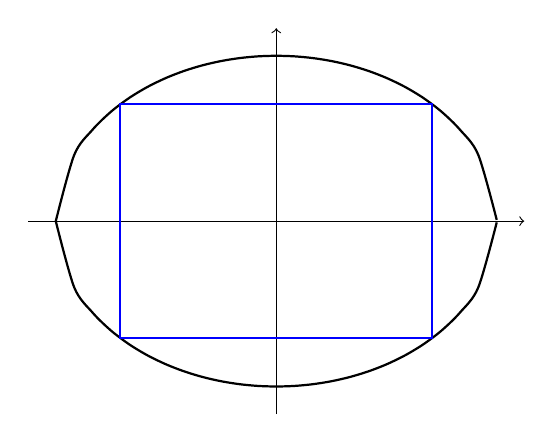
\begin{tikzpicture}[scale=0.7]
  \draw[->] (-4.5,0) -- (4.5,0);
  \draw[->] (0,-3.5) -- (0,3.5);
  \draw[thick] plot[smooth,domain=-4:4] (\x,{3*sqrt(1-\x*\x/16)});
  \draw[thick] plot[smooth,domain=-4:4] (\x,{-3*sqrt(1-\x*\x/16)});
  \draw[thick,blue] (-2.83,-2.12) rectangle (2.83,2.12);
\end{tikzpicture}
\hspace{0.6cm}
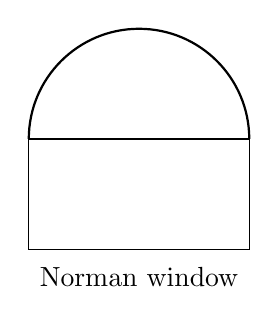
\begin{tikzpicture}[scale=0.7]
  \draw (0,0) rectangle (4,2);
  \draw[thick] (0,2) arc[start angle=180,end angle=0,radius=2];
  \node at (2,-0.5) {Norman window};
\end{tikzpicture}
\hspace{0.6cm}
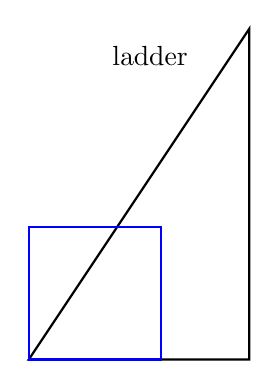
\begin{tikzpicture}[scale=0.7]
  \draw[thick] (0,0)--(4,0)--(4,6)--cycle;
  \draw[thick,blue] (0,0) rectangle (2.4,2.4);
  \node at (2.2,5.5) {ladder};
\end{tikzpicture}
\end{center}

\begin{center}
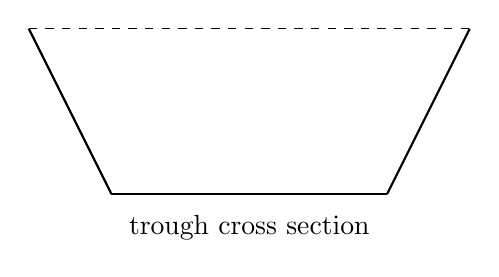
\begin{tikzpicture}[scale=0.7]
  \draw[thick] (0,0)--(5,0);
  \draw[thick] (0,0)--(-1.5,3);
  \draw[thick] (5,0)--(6.5,3);
  \draw[dashed] (-1.5,3)--(6.5,3);
  \node at (2.5,-0.6) {trough cross section};
\end{tikzpicture}
\hspace{0.8cm}
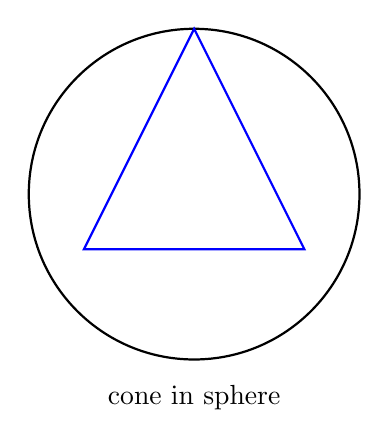
\begin{tikzpicture}[scale=0.7]
  \draw[thick] (0,0) circle (3);
  \draw[thick,blue] (0,3)--(-2,-1)--(2,-1)--cycle;
  \node at (0,-3.7) {cone in sphere};
\end{tikzpicture}
\hspace{0.8cm}
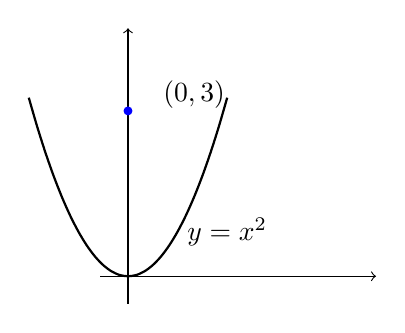
\begin{tikzpicture}[scale=0.7]
  \draw[->] (-0.5,0)--(4.5,0);
  \draw[->] (0,-0.5)--(0,4.5);
  \draw[thick,domain=-1.8:1.8,smooth] plot(\x,{\x*\x});
  \filldraw[blue] (0,3) circle (2pt);
  \node at (1.2,3.3) {$(0,3)$};
  \node at (1.8,0.8) {$y=x^2$};
\end{tikzpicture}
\end{center}

\section*{Answers}
\begin{enumerate}[leftmargin=*, itemsep=0.7em]
  \item $\displaystyle 4\sqrt{2}\times 3\sqrt{2}$
  \item width $=2\sqrt{3}$, height $=12$
  \item window width $=\dfrac{48}{4+\pi}$, rectangular height $=\dfrac{24}{4+\pi}$
  \item base side $=8\sqrt[3]{3}$, height $=4\sqrt[3]{3}$
  \item $r=5\sqrt[3]{2}$, $h=10\sqrt[3]{2}$
  \item page dimensions $=12$ by $18$
  \item triangle perimeter $=\dfrac{90\sqrt{3}}{\pi+3\sqrt{3}}$, circle circumference $=30-\dfrac{90\sqrt{3}}{\pi+3\sqrt{3}}$
  \item $x=10-2\sqrt{7}$
  \item $h=\dfrac{4R}{3}$
  \item bend angle satisfies $\cos\theta=\dfrac{\sqrt{3}-1}{2}$, so $\theta=\arccos\!\left(\dfrac{\sqrt{3}-1}{2}\right)$
  \item rectangle dimensions $=5\sqrt{2}$ by $5\sqrt{2}$
  \item closest points are $\left(\pm\sqrt{\frac52},\frac52\right)$
\end{enumerate}

\end{document}
